%----------------------------------------------------------------------------
\chapter{Mérési eredmények}
\label{sec:meresek}
%----------------------------------------------------------------------------
Az algoritmusok működését a saját laptopomon, egy virtuális gépen teszteltem, VirtualBox segítségével. Adataik:\\
\begin{center}
	\begin{tabular}{ll}
		\hline
		\textbf{Gép} & \\
		\hline
		Operációs rendszer & Windows 10 Pro\\
		Processzor & Intel(R) Core(TM) i3-3217U CPU @ 1.80GHz\\
		Memória (RAM) mérete & 4 GB\\
		\hline
		\textbf{Virtuális gép} & \\
		\hline
		Név & StochOpt\\
		Operációs rendszer & Ubuntu (64-bit)\\
		Alapmemória & 2549 MB\\
		SATA port 0 & StochOpt.vdi (Normál, 10 GB)
	\end{tabular}
\end{center}

A Szakdolgozat nevű image-ben telepítve lett az összes futtatáshoz szükséges csomag és alkalmazás. Ezeket a következő utasításokkal értem el:
\begin{lstlisting}
molnar@molnar-VirtualBox:~$ sudo apt-get install python-pip

molnar@molnar-VirtualBox:~$ pip install bayesian-optimization
molnar@molnar-VirtualBox:~$ sudo apt-get install mono-complete

molnar@molnar-VirtualBox:~$ clone https://github.com/GPflow/GPflowOpt
molnar@molnar-VirtualBox:~$ sudo pip install . --process-dependency-links

molnar@molnar-VirtualBox:~$ sudo add-apt-repository ppa:shogun-toolbox/nightly
molnar@molnar-VirtualBox:~$ sudo apt-get install python-shogun

molnar@molnar-VirtualBox:~$ sudo apt-get install default-jdk junit maven
\end{lstlisting}

\section{Modellek}
A tesztelést az alábbi modellekkel végeztem, melyek részletei \aref{sec:fuggelek} függelékben találhatóak.\\
\begin{center}
	\begin{tabular}{lcc}
		\textbf{Modell} & \textbf{Paraméterek} & \textbf{Reward függvények} \\
		\hline
		simple-server.pnml & 2 & 2 \\
		vcl\_stochastic.pnml & 7 & 7 \\
		hybrid\_cloud.pnml & 10 & 4\\
		philosophers\_3.pnml & 3 & 3\\
		philosophers\_5.pnml & 5 & 5\\
		philosophers\_7.pnml & 7 & 7\\
		philosophers\_9.pnml & 9 & 9\\
	\end{tabular}	
\end{center}


A következőekben \aref{sec:optimalizacios-megkozelitesek}. fejezetben felállított szempontrendszer szerint értelmezem és értékelem a különböző algoritmusok működését a mérések eredménye alapján.

%----------------------------------------------------------------------------
\section{Futási idő}
%----------------------------------------------------------------------------
A tesztesetek futási idejéről csak óvatosan tudunk következtetéseket levonni. Az eredmények alapján nemcsak a modellek nagysága, de főként a bonyolultsága is nagyban befolyásolja az egyes algoritmusok futási idejét, melyről így nem állapítható meg lineáris kapcsolat. Szintén, nem meglepő módon, nagy befolyásoló tényező az is, hogy az algoritmusok milyen pontokban kérdezik le a modell értékét, a megoldó keretrendszer válaszideje nagy változékonyságot mutat, a másodperc töredékétől akár 20 percig is terjedhet. A mérések átlagos alakulását \aref{fig:exectime}. ábra szemlélteti.
\begin{figure}[!ht]
	\centering
	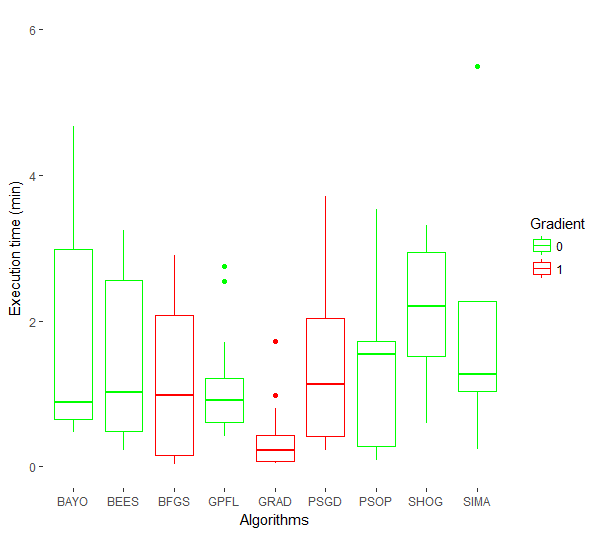
\includegraphics[width=140mm, keepaspectratio]{figures/execution_times_dobozdiagram.png}
	\caption{Algoritmusok átlagos futási ideje}
	\label{fig:exectime}
\end{figure}

Feltűnő a gradiens metódus átlagos futási idejének alacsony értéke, ez azonban csak annak tudható be, hogy az algoritmus, ha nem értelmezhető pontban szeretné kiszámolni az értéket, újraindul egy másik véletlen kezdőpontról, addig, míg el nem fogy a próbálkozásaink adott száma. Ennek a következményét a \aref{fig:derivaltak}. ábrán láthatjuk is.

Jelenleg a leglassabbnak a Shogun toolbox-szal való Bayesi optimalizálás, illetve a részecske raj és a szimulált lehűtés. Nem kell azonban elkeserednünk, a további szempontok alapján tisztább képet alkothatunk az algoritmusokról.
%----------------------------------------------------------------------------
\section{Deriváltak használata}
\label{sec:derivaltak}
%----------------------------------------------------------------------------
Gradiens számítást az L-BFGS, a gradiens módszer és a részecske raj optimalizáció gradiens módszerrel való ötvözése igényel. Kérdés azonban, hogy mennyire jobb ezek hatékonysága a többi algoritmushoz képest?

Az mérési eredmények pontosságát \aref{fig:derivaltak} dobozdiagrammon láthatjuk, összehasonlítva a deriváltakat használó és nem használó algoritmusokat. Az y tengely jelenti a mérés végeredményeként kapott pontban a célfüggvényünk értékét, a négyzetes hibaarányt. Azok tehát a leghatékonyabbak, melyek a legközelebb helyezkednek el a nullához.

A gradiens módszer hamar kiesett a sorból, hisz nem tud mit kezdeni a nem értelmezhető pontokkal, a szimulált lehűtés véletlen pontokba való ugrálása pedig a bonyolult, nagy dimenziószámú modelleknél nem bizonyul hatékonynak. Úgy tűnik, a mi sztochasztikus eseteinkben még a közkedvelt L-BFGS algoritmus is elvesztette a versenyt, hiába rendelkezik a gradiens számítás látszólagos előnyével. A gradiens számítás lényege valójában csak a részecske raj optimalizációnál nyilvánul meg egyértelműen: a gradienst ismerő raj algoritmus átlagosan az optimumhoz közelebbi értékeket talált, mint az egyszerű függvényszámítást végző társai.


\begin{figure}
	\centering
	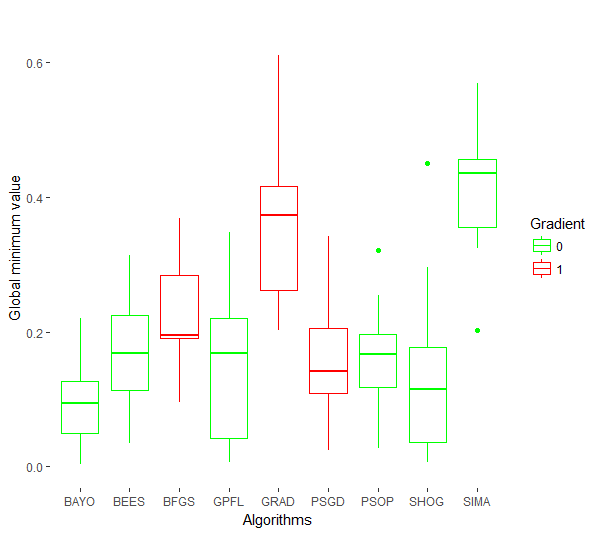
\includegraphics[width=140mm, keepaspectratio]{figures/gradiens_pontossag_boxplot.png}
	\caption{Optializáció átlagos pontossága algoritmusonként}
	\label{fig:derivaltak}
\end{figure}

Az algoritmusok átlagos számítási igénye \aref{fig:funccalc} dobozdiagrammon látszik. Az y tengely értéke jelzi, hányszor hívták meg átlagosan a megoldó keretrendszer kiértékelését egy adott paraméter lekötéssel az algoritmusok.

Itt már gyönyörűen látszik a Bayesi optimalizációk elsöprő sikere. Az ő eseteikben csak azok a hívások történnek, melyek a kezdeti feltérképező pontok, majd iterációnként egy újabb pont kiszámítását jelentik, mellyel a regressziós ill. klasszifikációs közelítő modellünket frissítjük. Ellentétben a nemkorlátos algoritmusokkal, melyek vagy rengeteg részecskét igényelnek az terület kellően alapos bejárására, vagy rengeteg iterációt az eredmény konvergálásához. Mint fentebb már volt róla szó, a gradiens módszer látszólagos hatékonyságát itt is az okozza, hogy nagyon hamar feladja a próbálkozást nem értelmezhető pontba való érkezéskor.

\begin{figure}
	\centering
	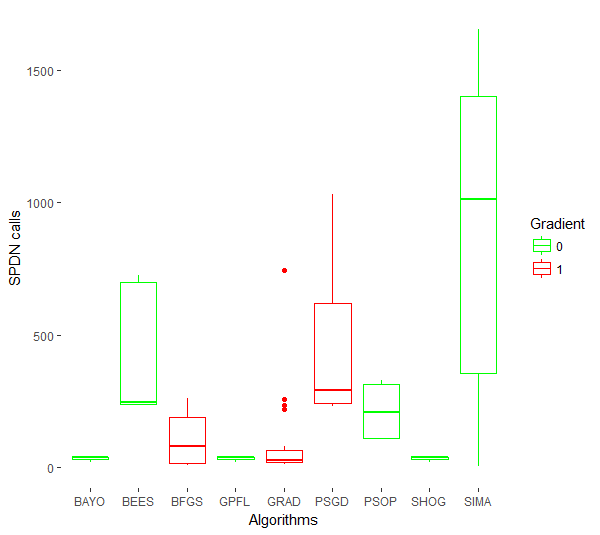
\includegraphics[width=140mm, keepaspectratio]{figures/func_calcs_boxplot.png}
	\caption{Megoldó keretrendszer hívásának száma algoritmusonként}
	\label{fig:funccalc}
\end{figure}

%----------------------------------------------------------------------------
\section{Hiperparaméterek}
%----------------------------------------------------------------------------
A mérésekben a legnagyobb nehézséget a sokféle algoritmus sokféle hiperparaméterének a beállítása jelentette. A változtatásuknak az eredménye helyenként megfeleltek a várakozásainknak, néhol azonban meglepő dolgokat tapasztalhatunk. Lássuk tehát a tanulságokat, mely paraméterek tűnnek dominánsnak az egyes algoritmusok esetében.
\paragraph{L-BFGS} \subparagraph{initPoint, restart} A hatékonyság leginkább azon múlik, megfelelő helyről indítjuk-e az algoritmust. Erről a "megfelelő" helyről azonban általában nincs tudomásunk, így minél többször indítjuk újra a futást, annál közelebb kerülhetünk az optimumhoz. Ezzel arányosan természetesen a futásidő is nő.
\paragraph{Gradiens módszer}\subparagraph{restart} Hasonló módon az L-BFGS-hez, a legnagyobb hasznot itt is a minél több próbálkozás hozza. Szerencsés esetben nagyon gyorsan tud az optimumba konvergálni, a mi nagy modelljeink esetében azonban az ilyen kezdőpont megtalálásának az esélye kevés.
\paragraph{Részecske raj}\subparagraph{swarmSize, maxIter, fiParticle, fiGlobal} Modellenként más és más képet mutatnak az eredmények, nem állapítható meg domináns hiperparaméter. Volt példa a raj számának, vagy az iterációk számának a növelésével némi javulásra, helyenként azonban a fi-k értékének a megváltoztatása két nagyságrendű javulást is eredményezett. Valóban látszik, hogy az optimalizáló algoritmusok nagy problémája, a megfelelő hiperparaméter beállítás minden modellre specifikus.
\paragraph{Részecske raj, gradiens módszerrel}\subparagraph{swarmSize, maxIter, fiParticle, fiGlobal, gradientMaxIter} Az alap algoritmushoz képest a gradiens módszer iterációszámának a növelése az elvárásoktól eltérően nem javítja jelentősen az eredményt. Úgy tűnik néhány lépéssel elég jól megközelíthető a lokális optimum, újabb iterációkkal nem számottevő a javulás. 
\paragraph{Méh algoritmus}\subparagraph{maxIter} Számos hiperparaméterrel rendelkező algoritmus, melyekre itt is fennáll, hogy modellenként változó hatékonyságot mutattak az ugyanolyan beállításaik. A kiemelkedő azonban ebben az esetben az iterációk száma volt. A növelésével jelentősebb javulások voltak elérhetőek, mint a többi paraméter állításával. Az algoritmus szépsége a felderítő és kizsákmányoló technika vegyítése, így nem meglepő, hogy minél tovább folytatjuk az algoritmus lépéseit, annál inkább feltérképezhető a függvénytér. Értelemszerűen ezért azonban nagy árat fizetünk, ahogy \aref{fig:funccalc}. ábrán is láthattuk.
\paragraph{Szimulált lehűtés}\subparagraph{$\emptyset$} Az  ábrázolt dobozdiagrammokon már láthattuk, hogy ez az algoritmus nem felel meg hatékonyságban az elvárásainknak. A mérési eredmények külön vizsgálásakor sem derül ki újabb információ. Hiperparaméter lehetőségei nem elég kifinomultak a mi modelljeink megfelelő mértékű optimalizálásához.
\paragraph{Bayesi optimalizálás, Scikit-learn csomaggal}\subparagraph{acq\_param, n\_iter, init\_points} Izgalmas dolgot tapasztalhatunk a nyereség függvény paraméterének a beállításakor. Ez a paraméter minél nagyobb, annál inkább tolódik az algoritmus a felderítő, és nem a kizsákmányoló módszer felé. A mi eseteinkben a felderítő technika hoz szembetűnő javulást, ami a kisebb modelleknél főként a futásidő drasztikus csökkenésében mutatkozik meg, a nagyobb modellek esetében azonban az optimumot is sokkal jobban megközelítik az ilyen beállítású mérések. Ezen kívül itt az iterációk és kezdőpontok száma közül az iterációk növelésével finomítható nagyobb mértékben a végeredmény.
\paragraph{Bayesi optimalizálás, TensorFlow-val}\subparagraph{init\_points} Bár kipróbáltam a jót sejtető kernel és nyereség függvény opciókat, semmilyen változást nem produkáltak. Több tizedesjegy nagyságban ugyanazokat a pontokat találták meg az algoritmus variánsok, csupán a futásidők különböztek, de azok sem szabályosan, valószínűsíthető, hogy ezt csak a keretrendszer válaszideje produkálta. Ami azonban kiderült, hogy ennél az implementációnál a kezdőpontok számán van a hangsúly! Minél több kezdeti ponttal állítjuk fel a becsült modellünket, annál precízebb eredményt kapunk, viszonylag kevés iterációszámmal is.
\paragraph{Bayesi optimalizálás, Shogun-toolbox-szal}\subparagraph{init\_points} Saját implementációjú Bayesi optimalizációmnak viszonylag kevés hiperparamétere van: a kezdőpontok és iterációk száma. A mérések során kiderült, hogy ebben az esetben is a kezdőpontok száma bír nagyobb befolyással a végeredményre, sokkal jobb hibaérték érhető el, és nem utolsó sorban a futási idő is barátságosabb, mint ha az iterációk számát növelnénk helyette.

%----------------------------------------------------------------------------
\section{Kényszerek implementálhatósága}
%----------------------------------------------------------------------------
A paraméterekre vonatkozó ismert korlátok kezelhetősége látványos különbséget mutat a nem korlátos és a Bayesi algoritmusok között. Ezek azok a korlátok, melyet a modellt ismerő szakértő tud megmondani a paraméterek értelmezési tartományáról. Hiszen egyértelmű, hogy egy időt jelölő paraméter nem vehet fel negatív értéket, vagy egy valószínűségi érték 1-nél nagyobb számot.

A nem ismert korlátok\footnote{black-box constraints} -- vagyis a függvénytér nem értelmezhető területeinek -- kezelésére a nemkorlátos algoritmusok esetén nem volt jó megoldásunk. Az L-BFGS, gradiens módszer és szimulált lehűtés esetén egyszerűen félbehagytuk az optimalizálást, és megpróbáltuk újrafuttatni az elejétől, másik kezdőpontból. A részecske raj algoritmusoknál ilyen esetben pedig csak egy konstans nagy értéket adtunk függvényértékül a részecskének, ezzel elkerülve a hosszas véletlenszerű próbálkozásokat minden részecske esetén, aki ilyen területre téved.

A mérési eredményekről egy átlagos képet mutatni ebben az esetben nem lenne praktikus, mivel az elvárt értékektől való eltérés egyes esetekben 20-30 nagyságrendnyi. Ehelyett  \aref{table:globalminimumpoints} táblázat egy-egy konkrét futási eredményt tartalmaz, melyből nagyságrendileg láthatjuk, az algoritmusok mennyire képesek megközelíteni az általunk elvárt globális minimum pontot, a különböző bonyolultságú modellek esetében.

Láthatjuk tehát, hogy bár a célfüggvény minimalizálása sok esetben hasonlóan jól sikerül (lásd: \ref{fig:derivaltak}. ábra), a talált, és az általunk várt minimumpont különbsége jól mutatja a Bayesi optimalizálás nagyszerűségét a többi, véletlenekre és gradiensekre alapuló algoritmussal szemben.

\begin{table}
	\fontsize{8}{9.5}\selectfont
	\center
	\begin{tabular}{ll}
		\hline
		\textbf{philosophers\_3} &\textit{(7.33, 2.15, 9.68)}\\
		\hline
		BFGS & (1.14E24, 2.54E7, 1.08E19)\\
		GRAD & (8.73E24, 2.39E8, 2.79E33)\\
		PSOP & (1.08E15, 120.01, 3.28E15)\\
		PSGD & (9.55E22, 10.12, 1.02E39)\\
		BEES & (1.59, 4.94E3, 29.9)\\
		SIMA & (2.12E24, 4.46E4, 7.87E31)\\
		BAYO & (7.34, 3.19, 77.71)\\
		GPFL & (54.6, 2.4, 80.1)\\
		SHOG & (25.67, 2.28, 14.54)\\
		\hline
		\textbf{philosophers\_5} & \textit{(7.33, 2.15, 9.68, 9.64, 9.47)}\\
		\hline
		BFGS & (2.14E20, 3.08E3, 7.74E16, 8.12E13, 2.09E16)\\
		GRAD & (8.66E16, 23.32, 4.66E15, 1.96E31, 1.07E33)\\
		PSOP & (1.4E12, 8.77E4, 2.53E12, 1.24E14, 2.83E23)\\
		PSGD & (1.35E12, 14.59E4, 4.13E12, 2.01E21, 1.17E23)\\
		BEES & (3.58E18, 1.18E6, 4.59E17, 1.66E17, 4.04E14)\\
		SIMA & (3.44E29, 7.63E2, 3.21E10, 1.44E24, 2.63E27)\\
		BAYO & (4.03, 13.72, 82.99, 15.61, 14.78)\\
		GPFL & (3.08, 13.17, 7.04, 7.04, 46.98)\\
		SHOG & (69.99, 0.96, 55.33, 18.74, 29.34)\\
		\hline
		\textbf{philosophers\_7} & \textit{(7.33, 2.15, 9.68, 9.64, 9.47, 4.03, 3.01)}\\
		\hline
		BFGS & (2.43E15, 5.51E7, 7.23E14, 1.57E9, 6.04E10, 2.82E15, 7.51E9)\\
		GRAD & --\\
		PSOP & (8.25E16, 8.96E2, 3.97E31, 3.13E26, 1.23E37, 3.75E7, 5.95E6)\\
		PSGD & --\\
		BEES & (6.79E19, 1.88E6, 3.53E22, 2.04E27, 5.88E20, 4.05E14, 4.42E9)\\
		SIMA & (2.89E9, 9.45E4, 2.11E19, 2.74E25, 3.75E37, 1.21E10, 7.69E4)\\
		BAYO & (69.29, 1.56, 88.98, 84.87, 3.31, 5.66, 6.27)\\
		GPFL & (12.50, 7.08, 45.45, 45.45, 2.74, 15.87)\\
		SHOG & (22.64, 1.83, 84.58, 11.99, 9.34, 24.52, 3.01)\\
		\hline
		\textbf{philosophers\_9} & \textit{(7.33, 2.15, 9.68, 9.64, 9.47, 4.03, 3.01, 1.24, 6.63)}\\
		\hline
		BFGS & (1.93E22, 14.03, 1.07E39, 6.67E32, 7.52E8, 1.46E17, 1.5E4, 2.67E3, 1.84E14)\\
		GRAD & (1.75E12, 5.889E5, 7.73E37, 1.22E26, 1.39E22, 2.54E11, 5.51E9, 14.87, 1.77E24)\\
		PSOP & (1.69E23, 29.23E2, 1.99E21, 1.17E11, 4.38E10, 1.64E7, 8.93E7, 126.0, 3.51E21)\\
		PSGD & (1.42E9, 7.58E4, 2.8E19, 1.67E29, 9.38E22, 1.39E15, 9.42E9, 5.43E2, 6.73E18)\\
		BEES & (1.62E7, 2.55, 6.51E33, 6.3E22, 4.53E22, 1.2E4, 8.36E7, 3.15, 4.31E22)\\
		SIMA & (2.79, 1.26E8, 7.79E37, 2.78E4, 2.62E29, 34.9, 7.74E12, 3.93E4, 3.08E17)\\
		BAYO & (0.80, 9.95, 89.34, 5.61, 80.63, 7.78, 1.9, 1.11, 59.96)\\
		GPFL & (5.47, 1.56, 7.04, 7.04, 10.11, 37.26, 7.46, 2.14, 31.32)\\
		SHOG & (40.59, 7.54, 129.4, 137.5, 18.91, 9.02, 0.85, 5.5, 16.55)\\
		\hline
		\textbf{simple-server} & \textit{(1.5, 0.25)}\\
		\hline
		BFGS & (1.5, 0.25)\\
		GRAD & (1.5, 0.25)\\
		PSOP & (14.08, 0.87)\\
		PSGD & (1.5, 0.25)\\
		BEES & (1.49, 0.25)\\
		SIMA & (1.49E3, 7.48)\\
		BAYO & (2.64, 0.74)\\
		GPFL & (3.27, 0.54)\\
		SHOG & (1.81, 0.68)\\
		\hline
		\textbf{vcl\_stochastic} & \textit{(0.015, 0.5, 0.15, 60, ., 0.75, 0.6)}\\
		\hline
		BFGS & --\\
		GRAD & --\\
		PSOP & --\\
		PSGD & --\\
		BEES & --\\
		SIMA & --\\
		BAYO & (0.02, 38.21, 10.63, 304.3, 499.8, 0.56, 0.66)\\
		GPFL & (0.78, 26.31, 7.1, 3.47E3, 289.5, 0.0075, 0.006)\\
		SHOG & (1.31, 21.32, 11.92, 594.8, 41.86, 3.89, 0.58)\\
		\hline
		\textbf{hybrid\_cloud} & \textit{(5, 0.75, 0.0002, 0.2, 0.1, 0.0002, 0.1, 24, 0.8, 0.3, 0.01, 1000)}\\
		\hline
		BFGS & --\\
		GRAD & --\\
		PSOP & (12.21, 1.48, 1.002, 1.27, 2.17, 1.001, 1.019, 1.52E11, 2.33, 1.68, 1.02, 1.67E-66)\\
		PSGD & --\\
		BEES & --\\
		SIMA & --\\
		BAYO & (3.69, 0.37, 0.0008, 0.11, 0.71, 0.0004, 0.05, 27.75, 0.67, 0.06, 0.009, 139.9\\
		GPFL & (2.42, 0.99, 0.0005, 0.26, 0.21, 0.0005, 0.02, 22.1, 0.38, 0.18, 0.06, 2084.2)\\
		SHOG & (2.8, 0.22, 0.002, 0.07, 0.97, 0.0003, 0.09, 29.81, 0.88, 0.97, 0.002, 1362.7)\\	
	\end{tabular}
	\caption{Talált globális minimum pontok modellenként és algoritmusonként}
	\label{table:globalminimumpoints}
	\begin{tablenotes}
		A bonyolultabb modellekkel sok algoritmus nem tudott megbírkózni, futásuk alatt nem találtak kiszámítható pontot. Ezeket -- jellel jelöltem a táblázatban
	\end{tablenotes}
\end{table}
%----------------------------------------------------------------------------
\section{Értelmezhető - nem értelmezhető területek aránya}
\label{sec:teruletek}
%----------------------------------------------------------------------------
Mivel fő célunk a sztochasztikus modellek optimalizálása, nem ismert korlátokkal, az algoritmusok hatékonyságát nagyban jellemzi, hogy a kiszámított pontok közül hány értelmezhető, és hány nem. Egy olyan algoritmust keresünk, ami megtalálja a kiszámítható területeket, és ott végez kimerítő keresést, ezáltal kevés számítást pazarolva a nem értelmezhető területekre.

A modellek közül a philosophers\_9.pnml egy azok közül, melyek optimalizálása során nagy számban futottak nem értelmezhető területekre az algoritmusok. Az átlagos eloszlását ezen területeknek \aref{fig:ertelmezhetopontok}. ábrán láthatjuk.

\begin{figure}[!ht]
	\centering
	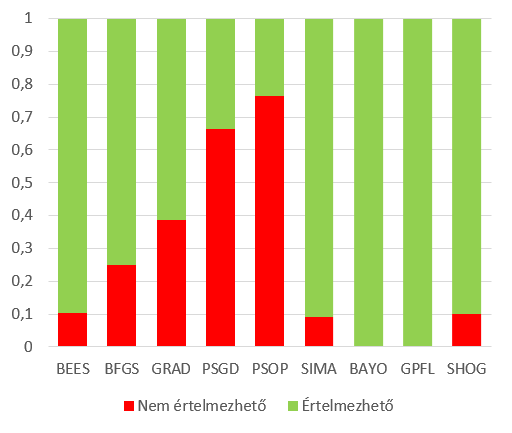
\includegraphics[width=140mm, keepaspectratio]{figures/fil9pontaranyok.png}
	\caption{Számítható és nem számítható pontok eloszlása az algoritmusokat a philosophers\_9 modellen futtatva}
	\label{fig:ertelmezhetopontok}
\end{figure}

A Bayesi algoritmusokat befolyásolni tudjuk az eddigi információink alapján. Erre két példát mutattak az implementációim: nem értelmezett pont értékén egy konstans nagy büntetőérték adása, mellyel biztatni szeretnénk a regressziós modellt arra, hogy itt ne keressen tovább minimumom, illetve a klasszifikáció eszközével, amikor egyértelműen tároljuk a kiszámított pontokról, értelmezhetőek-e, vagy sem, és ennek a valószínűsége is szerepet játszik a nyereség függvényben. Ennek az eredményessége egyértelműen látszik a halmozott oszlopdiagrammon, bár sajnálatos, hogy a klasszifikáció megvalósítása a MyShogunOpt osztályban még nem olyan hatékony, mint a GPFlowOpt és a BayesianOptimization Python implementációké.
%----------------------------------------------------------------------------
\section{Összehasonlítás}
%----------------------------------------------------------------------------
